% ****** Start of file RamanCoolingV1.tex ******
%
%
% See the REVTeX 4 README file
% It also requires running BibTeX. The commands are as follows:
%
%

\documentclass[%
 reprint,
%superscriptaddress,
%groupedaddress,
%unsortedaddress,
%runinaddress,
%frontmatterverbose, 
%preprint,
%showpacs,preprintnumbers,
%nofootinbib,
%nobibnotes,
%bibnotes,
 amsmath,amssymb,
 aps,
prl,
%pra,
%prb,
%rmp,
%prstab,
%prstper,
%floatfix,
]{revtex4-1}

\usepackage{graphicx}% Include figure files
\usepackage{dcolumn}% Align table columns on decimal point
\usepackage{bm}% bold math
%\usepackage{hyperref}% add hypertext capabilities
%\usepackage[mathlines]{lineno}% Enable numbering of text and display math
%\linenumbers\relax % Commence numbering lines

%\usepackage[showframe,%Uncomment any one of the following lines to test 
%%scale=0.7, marginratio={1:1, 2:3}, ignoreall,% default settings
%%text={7in,10in},centering,
%%margin=1.5in,
%%total={6.5in,8.75in}, top=1.2in, left=0.9in, includefoot,
%%height=10in,a5paper,hmargin={3cm,0.8in},
%]{geometry}

\begin{document}

%\preprint{APS/123-QED}

\title{A Plugged Trap for Crossed Field Spin-Flip Loss}%


\author{David Reens}%
\author{Hao Wu}
\author{Tim Langen}%
\author{Jun Ye}
\affiliation{%
 Physics Department, University of Colorado at Boulder\\
}%

\date{\today}% It is always \today, today,


%%%%%%%%%%%%%%%%%%%%%
%ABSTRACT
%%%%%%%%%%%%%%%%%%%%%
\begin{abstract}
A new electromagnetic trap geometry allows tunable plugging of non-adiabatic spin flip loss in crossed electric and magnetic fields. This loss afflicts a wide set of candidate molecules and operates at much higher temperatures compared with the more familiar atomic spin-flip loss near the zero of a magnetic trap, and thus it's removal represents an important step toward ultracold molecules. Using only an external magnetic bias coil, the loss rate is tuned from over $100 \text{ s}^{-1} $ to below the vacuum limited lifetime of $2 \text{s}^{-1}$ in a $100 \text{ mK}$ sample of OH molecules.
\end{abstract}


\maketitle


%%%%%%%%%%%%%%%%%%%%%%%%%%%%%%%%%
%
%     III   NNN   TTT   RRR   OOO   DDD   UUU   CCC   TTT   III   OOO   NNN
%     III   NNN   TTT   RRR   OOO   DDD   UUU   CCC   TTT   III   OOO   NNN
%     III   NNN   TTT   RRR   OOO   DDD   UUU   CCC   TTT   III   OOO   NNN
%
%%%%%%%%%%%%%%%%%%%%%%%%%%%%%%%%%
%\section{Introduction}
The ultracold regime extends toward molecules on many fronts. Several bialkali molecules are available and others are under development. Creative and carefully engineered laser cooling strategies are tackling certain nearly rotationally diagonal molecules. A plethora of non-optical cooling strategies have succeeded to greater or lesser extents on other molecules. All of these molecules will require secondary strategies like evaporation or sympathetic cooling to make further gains in phase space density. They also may face a familiar challenge: spin flip loss near the zero of a magnetic trap, only dramatically enhancemed for certain molecules. Here we report on our encounter with OH molecule enhanced spin flip loss and our solution.

The knowledge of spin flips or Majorana hops as an eventual trap lifetime limit predates the very first magnetic trapping of neutrals\cite{Migdall1985}. Spin flips were directly observed and overcome in the TOP trap\cite{Petrich1995}, and shortly later with a plugged dipole trap\cite{Davis1995}, famously enabling the first Bose-Einstein condensates. The molecular spin-flips can occur at much higher temperatures compared with their atomic counterpart, and thus they need to be addressed much earlier than might have been expected. The magnitude of the loss varies with molecular species, and is particularly strong for the case of the neutral hydroxyl radical (OH) that we study. 

Essentially, the loss enhancement is related to the sensitivity of molecules not only to the rotation of the magnetic field in the trap, but also to the relative orientation of electric and magnetic fields. For Hund's case (a) molecules with very strong spin-rotation coupling, or for case (b) molecules to the extent that their spin-rotation coupling $\gamma$ is nonzero, electric and magnetic fields add linearly when the fields are parallel but sublinearly when the fields are orthogonal. We call this ``blocking". The presence of a constant orthogonal electric field blocks the magnetic field so that the Zeeman splitting is reduced. For ground state $^2\Pi_{3/2}$ weak field seeking OH, the Zeeman splitting is blocked from linear to cubic as shown in fig.~\ref{fig:blocking}. Since the orthogonal electric field couples opposite spin states, if these are three quanta apart as for the highest state in a $J=3/2$ manifold, the Zeeman splitting is heavily blocked from linear to cubic. This blocking means that when $B<<E$ and $B\cdot E=0$ are met, the energy gap between the highest two states is small, and spin-flips can occur. In a quadrupole trapping geometry with homogeneous electric field, these conditions are met on a disk  through the origin whose size is controlled by the magnitude of $E$. Just outside the disk, blocking returns to linear, which results in a worst case scenario for loss, since $P_{\text{flip}}\propto e^{-\Delta^2/(dE/dt)}$ and we have not only small $\Delta$ but large $dE/dt$. Panel (e) of fig.~\ref{fig:blocking} describes this further.

\begin{figure}
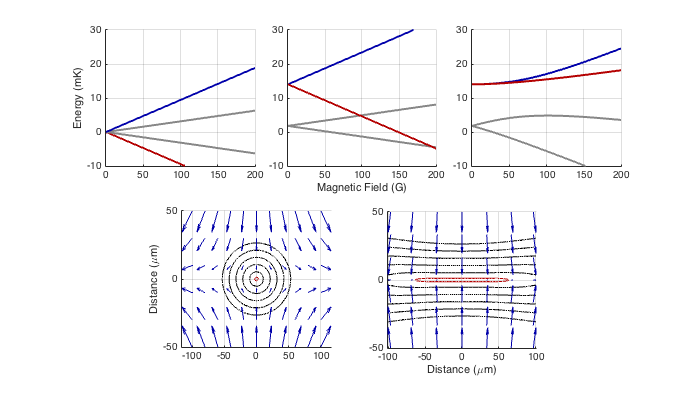
\includegraphics[width=100mm]{blocking.png}%
\caption{
The blocking effect. (a), four Zeeman split lines in the ground state of OH. A nearly identical set of four states of opposite parity lie 100 mK below. The trapped state and it's spin flip partner are in blue and red. (b) Zeeman splitting with the addition of an electric field of 150 V/cm parallel to the magnetic field. (c) Again but with the fields orthogonal. (d) Contours showing the gap between blue and red states near the zero of a magnetic quadrupole trap without electric field. (e) Again with 150 V/cm. Note the drastic widening of the lowest contour, but without gradient reduction nearby.
\label{fig:blocking}}
\end{figure}

\begin{figure*}
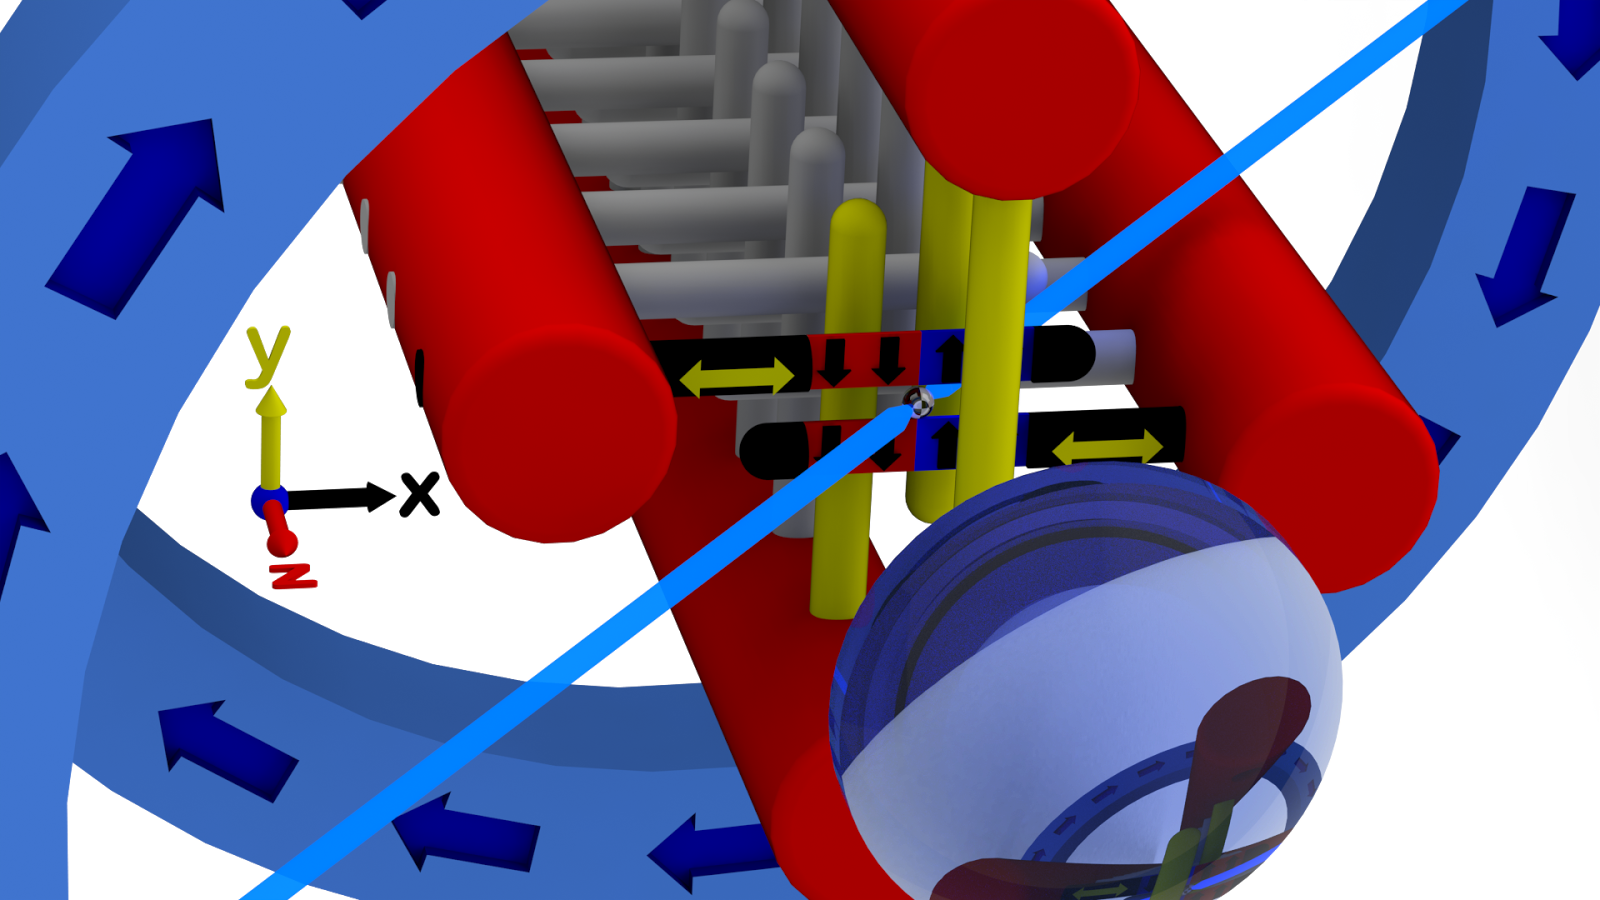
\includegraphics[width=180mm]{blue-red-yellow-v2_CAD.png}%
\caption{
OH molecules are created using a supersonic expansion source and decelerated from an initial velocity of 460m/s to a final velocity of 40ms/s using a Stark decelerator (red). The decelerator contains 142 electrode pairs (gray). Trapping is achieved by combining a radial magnetic quadrupole field, created by the magnetized second to last electrode pair of the decelerator, with a longitudinal electric quadrupole field created by the third to last and last electrode pairs, respectively (yellow, one electrode is omitted for clarity). The magnetized electrodes can be translated in situ along the x-axis to align their domains and optimize the quadrupole. As there is no trapping magnetic field in the z-direction in this configuration, macroscopic external bias coils can be used to lift the gap between the top two states of the OH ground-state manifold and thus tune the molecular loss. Detection is realized using laser induced fluorescence along the x+y-z direction (blue), which is collected using a lens system and PMT in the z-direction.
\label{fig:CAD}}
\end{figure*}

We can apply Brillouin-Wigner perturbation theory or analytically solve the ground state eigenenergies and taylor expand to obtain the following functional form for the gap between the states where $E\cdot B=0$:

\begin{equation}
\label{eq:HZprop}
H_Z\propto \frac{B^3}{E^4}\Delta^2
\end{equation}

\noindent Here $B$ and $E$ are field strengths converted to units of energy using the magnetic moment $\mu_B$ and the electric dipole moment $d_E$ respectively. Of course the whole point we are making relates to the fact that the potential energy of the molecule does not scale linearly with these fields, but it still adds clarity to our expressions to express fields in energy units via the constants taken from the linear Zeeman and Stark regimes. We can use this to develop a scaling law for the enhancement. Let $\kappa$ be the energy threshold for gaps between states below which spin-flips are possible at the 50\% level. $\kappa$ depends on the mean velocity of trapped species and on the trap gradient, and so must be separately computed for any given scenario. For OH molecules in the quadrupole trap described here \cite{} with gradient $4T/cm$ and temperature $50mK$, $\kappa=5\text{MHz}$. Without electric field, the effective cross sectional area for a hopping region is $\pi \kappa^2$, since loss can occur where $B<\kappa$. With electric field, a much larger $B$ field is required to overcome blocking, so we have from eq.~\ref{HZprop} that $B < \sqrt[3]{\frac{\kappa E^4}{\Delta^2}}$, so for $E>\sqrt{\kappa\Delta}$ there is an enhancement given by the following equation:
\begin{equation}
\nu = \left(\frac{E^4}{\kappa^2\Delta^2}\right)^\frac{2}{3}
\label{eq:blimit}
\end{equation} 

The following table provides numerical values of the loss enhancement factor and absolute rates for various conditions of experimental interest for OH molecules.

\begin{table}[h]
\caption{Enhancements and Rates for OH molecules}
\label{tab:rates}
\begin{tabular}{c|ccc}
\toprule
E & $\nu$ & $\Gamma$ & Purpose \\
\toprule
10 V/cm & 1 & 1 & Stray Field \\
300 V/cm & 10 & 10 & Evaporation Crossings\\
550 V/cm & 20 & 20 & Spectroscopy Crossings\\
3 kV/cm & 100 & 100 & Polarizing Field\\
\toprule
\end{tabular}
\end{table}

It is interesting to note that in ref.~\cite{Lara2008}, it was specifically undertaken to investigate the spin-flip loss for OH molecules in a magnetic quadrupole trap with superposed electric field, and no enhancement was found. This turns out to be a consequence of a reasonable yet false assumption that a 4-state approximate Hamiltonian with two spin states and two parities would contain the behavior relevant for spin-flip loss in mixed fields. This approximate Hamiltonian exhibits only constant order blocking- i.e. the Zeeman effect remains linear though with adjusted slope. C.f. the gray $M_J=\pm1/2$ state curves in panel (c) of fig.~\ref{fig:blocking}.

%%%%%%%%%%%%%%%%%%%%%%%%%%
%  PIN TRAP GEOMETRY
%%%%%%%%%%%%%%%%%%%%%%%%%%


One obvious way to avoid the loss enhancement is to simply never use electric field in a magnetic trap. This prevents loss from being enhanced compared with atoms, but doesn't remove it entirely. Another possibility is to trap with electric fields, where no spin-flip loss is possible thanks to the large lambda-doublet splitting. However this splitting also results in a significant reduction in trap gradient close to the trap center, very undesirable for further cooling by evaporation, which needs as much phase space density as possible.


Seeking to remove the loss entirely but without trap gradient sacrifice, we switch from a 3D to a 2D magnetic trap, and use electric fields to trap in the remaining dimension. This does not remove the possibility of $E.B=0$, but it allows us to tune the minimum magnetic field with an external bias coil oriented along the zero axis of the 2D quadrupole trap.  Our fields are as follows:
\begin{eqnarray}
\vec{B} &=&  B^\prime y\hat{x}+ B^\prime x\hat{y} + B_{coil} \hat{z}\\
\vec{E} &=&  E^\prime y\hat{y}-  E^\prime z\hat{z}
\end{eqnarray}

\noindent In other words 2D quadrupole traps in the xy plane for B and in the yz plane for E. Serendipitously, we are able to achieve these fields with a geometry that exactly matches that of our Stark decelerator, as shown in fig.~\ref{fig:CAD}. This represents a near best-case scenario for coupling between a pulsed decelerator and a trap. For N38 magnets chosen so as to maintain magnetization during violent conditioning procedures, $B^\prime=5 T/cm$ and $E^\prime=?$. These correspond to trap frequencies for a molecule with velocity matching the thermal mean of $7m/s$ of $\nu=?$ in each direction.

\begin{figure}
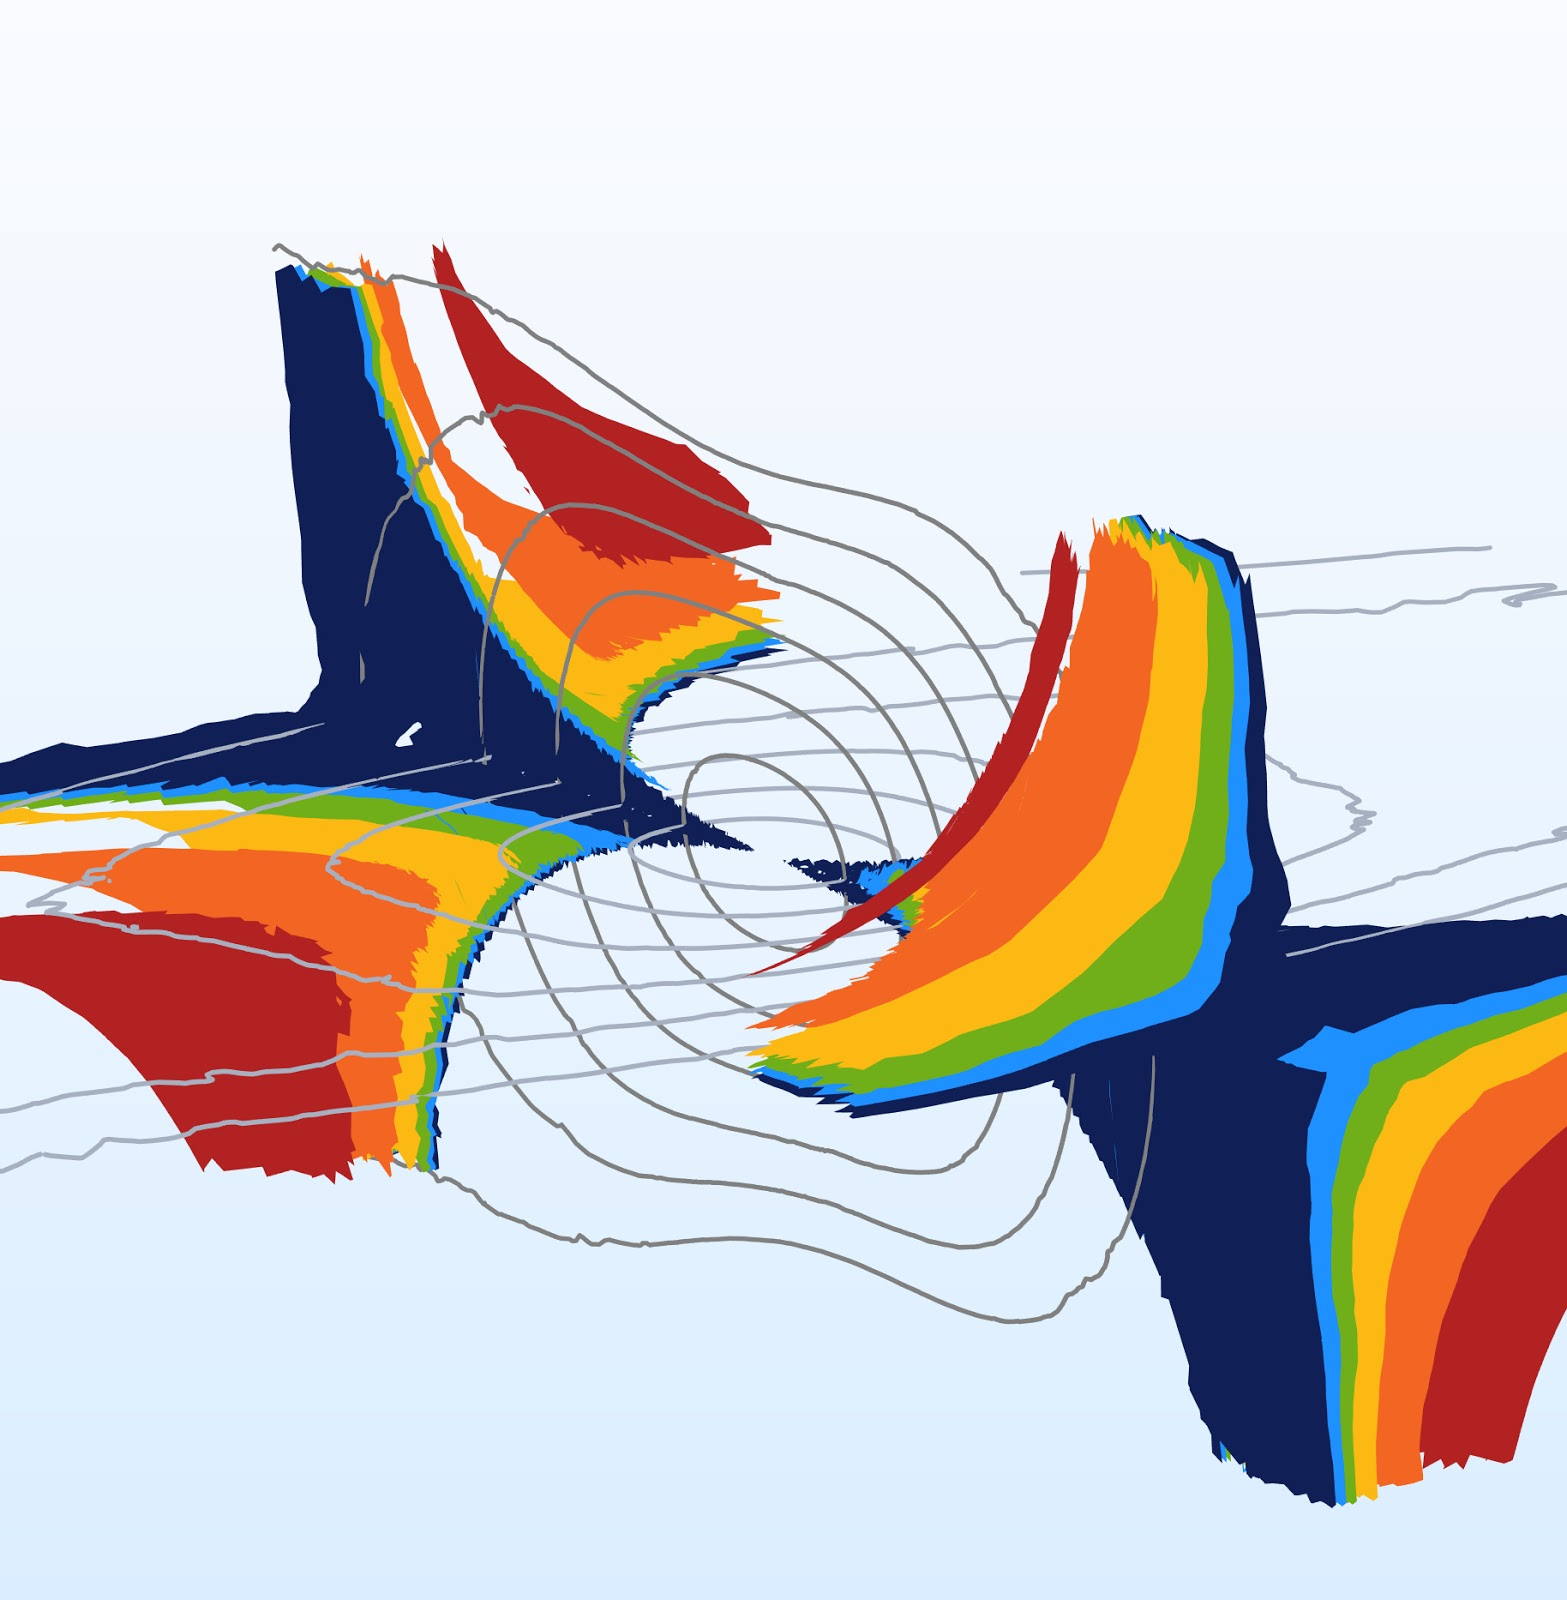
\includegraphics[width=90mm]{Loss_Surface_Chunks_0-320_0.jpeg}%
\caption{
Contours every 100mK, colors 0,20,40,80,160,320 G bias field and pin offset at zero. Molecules can spin-flip and be lost, whenever they cross these areas.
\label{fig:LSurfs}}
\end{figure}

Now regarding the molecule enhanced spin-flip loss, E is perpendicular to B when:
\begin{eqnarray}
\vec{B}\cdot \vec{E} &= 0\\
B^\prime x E^\prime y - B_{coil}  E^\prime z &= 0\\
B_{coil}z &= xyB^\prime
\end{eqnarray}

So we see that E and B are perpendicular on a hyperbolic sheet which deviates more significantly from the z axis with increasing $B_{coil}$, and reduces to the pair of planes $x=0$ and $y=0$ in the limit that $B_{coil} = 0$. On this hyperbolic sheet, $B$ must be larger than the threshold set by Eq.~\ref{eq:blimit} to overcome blocking. Fortunately, $B_{coil}$ does not have to overcome the blocking limit, it only needs to push the $B\cdot E=0$ surfaces slightly away from the z-axis for the strong magnetic quadrupole fields to overcome the blocking. In fig.~\ref{fig:LSurfs}, the surfaces where $E\cdot B=0$ are colored wherever the gap there is below the threshold $\kappa$, for several different choices of $B_\text{coil}$. Since the magnetic fields are more localized than the electric, there are always regions susceptible to spin flips, but they can be pushed far enough from the trap center so as to only affect molecules which could already escape the trap by mechanical means. 

\begin{figure}
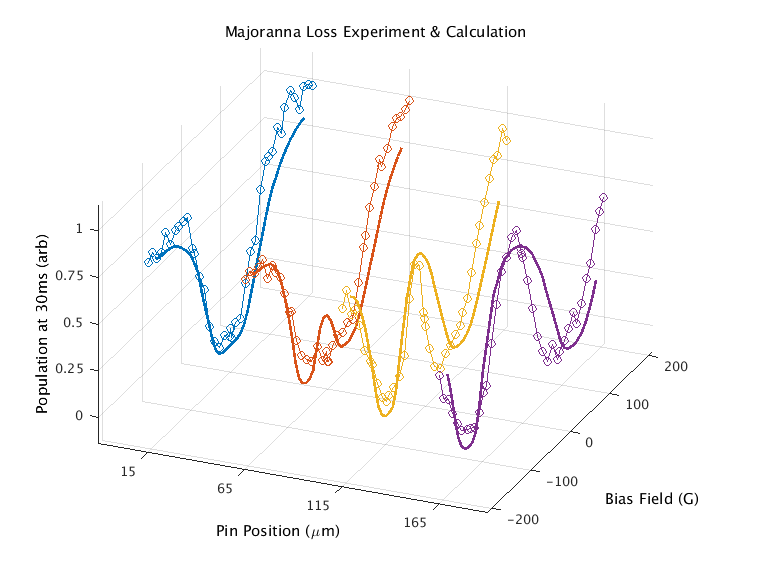
\includegraphics[width=90mm]{V-to-W-plot-3D-dave.png}%
\caption{
Family of curves showing the remaining population after $30 \text{ms}$ as a function of pin offset and magnetic bias field.
\label{fig:WVplot}}
\end{figure}

In fact, from fig.~~\ref{fig:LSurfs} it would appear that $B_{coil}$ essentially tunes the proximity of the loss regions to the trap center, and that for $B_{coil}$ large enough the loss should be removed. However, after some failed experimental attempts and a careful consideration of potential deviations from our target geometry, we realized that translations of our magnetic pins in their mounts lead to important modifications to the axial behavior of the magnetic trap. Essentially, when the pairs of magnetic domains of the two pins are out of mutual alignment by a distance $d$, a small trapping field $\vec{B}\propto B^\prime z\hat{z} d$ is introduced. This means that $B_\text{coil}$ no longer directly tunes the minimum magnetic field in the trap. Instead, $B_\text{coil}$ must first overcome the slight trapping field along the $z$-axis, moving a region of zero field along the z axis and eventually out of the trap. In order to really disentangle this effect from our results, we installed an in-situ pin translation stage and obtained the family of curves shown in fig.~\ref{fig:WVplot}. With the pins tuned nearly into alignment, the magnetic field does indeed tune reduce the loss in either direction of tuning. Otherwise, magnetic field first increases the loss by moving the magnetic zero into regions of large electric field, but eventually overwhelms it, leading to a characteristic double-well shape. 

We fit the family of curves shown in fig.~\ref{fig:WVplot} by performing a detailed numerical integration of Landau-Zener hopping probability over all hyperbolic planes where loss can occur, weighted by the expected Maxwell-Boltzmann distribution of molecules in the trap. The computation is performed in COMSOL Multiphysics, with cloud temperature and magnet strength as the only free parameters. Source-code for the model is available.\cite{ref:githubCOMcode} The fit temperature is $100\pm10\text{ mK}$, and the magnetization is $1.2\pm0.1\text{T}$, where the uncertainties are chosen so as to keep the fit $R^2$ within a factor of $2$ of the optimal. This temperature is twice that of our previous traps, most likely due to the increased trap depth. The magnetization is consistent with our expectations of the NdFeB magnet grade selected.

\begin{figure}
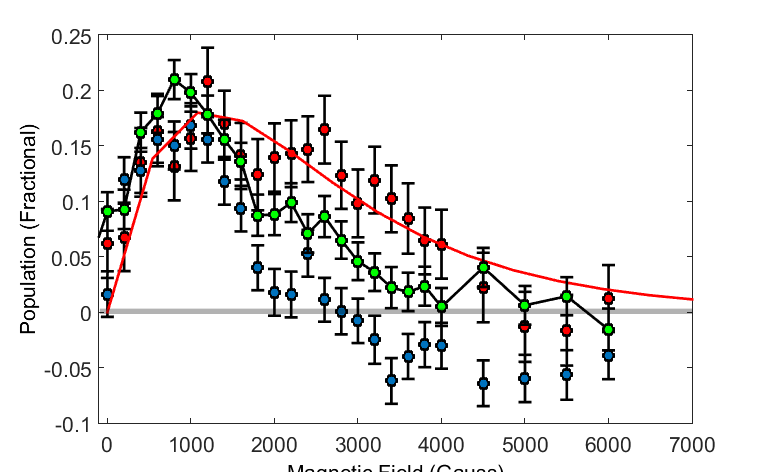
\includegraphics[width=90mm]{MW-thermometry.png}%
\caption{
Microwave Thermometry in the trap.
\label{fig:spec}}
\end{figure}

As a further confirmation of our model for the spin-flip loss in this trapping geometry, we perform a Zeeman spectroscopy along the $f 3/2$ to $e 3/2$ line as in our previous work \cite{?} to measure the population fraction as a function of magnetic field. The results are shown in fig.~\ref{fig:spec}. With the magnetic pins aligned, it is seen that higher values of $B_{\text{coil}}$ increase the population of molecules accessing higher magnetic fields in the trap. This is consistent with our expectation that $B_\text{coil}$ would tune the distance of the loss region from the trap center. In order to perform this spectroscopy, the trapping electric fields are switched off immediately prior to the application of a microwave transfer pulse tuned to a particular magnetic field strength. Thus the results only reflect the Zeeman potential energy of the molecules, not the Stark. 

It is interesting to note that in the case of lowest applied magnetic field in fig.~\ref{fig:spec}, i.e. deepest cutting of the loss region toward the trap center, a negative going signal is observed. Since the population signal is obtained via subtractive comparison of molecules in the $f 3/2$ state with and without a coupling from $f 3/2$ to $e 3/2$ applied at a particular magnetic field, this indicates that the coupling actually restored molecules from $e 3/2$ to $f 3/2$. This observation is consistent with the existence of a secondary trapped state whose state character in the $JM\Omega\epsilon$ basis includes regions of $e$ parity. Since this state connects to the primary doubly-stretched state that is weak field seeking with respect to both fields by magnetic spin flips, it would seem that it ought to be magnetically strong field seeking and thus un-trapped. However, this strong field seeking behavior only persists in a small region of magnetic field before crossings with the $f 1/2$ state and later the $e 3/2$ state facilitate adiabatic transitions to states which retain magnetically weak field seeking character. 

\begin{figure}
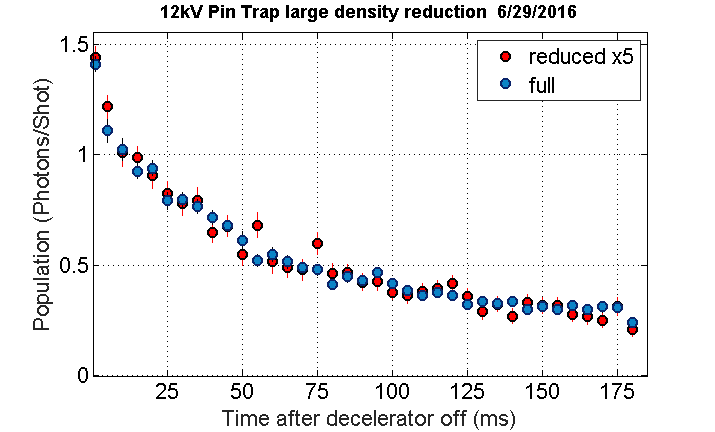
\includegraphics[width=90mm]{reduce-density-compare.png}%
\caption{
Trajectory over time with loss removed, with and without a density reduction technique.
\label{fig:timetrace}}
\end{figure}

We have conclusively demonstrated the existence of molecule enhanced spin-flip loss by tuning it from an overwhelming rate to complete removal. It remains to be seen what other processes may be in effect once this loss mechanism is removed. Although the trend shown in fig.~\ref{fig:timetrace} is suggestive of a collisional process, we implement a completely phase-space blind density reduction technique to significantly reduce our molecule number and observe no change in the trend, indicating that only single particle physics is responsible so far. This is not too surprising given the increased initial temperature of this trap compared to our previous ones, but we intend to address this with a suite of density enhancing experimental improvements in the near term.

%includes uncited bib entries
\nocite{*}


\bibliography{MolecularMajoranaLoss.bib}% Produces the bibliography via BibTeX.

\end{document}
%
% ****** End of file MolecularMajoranaLoss.tex ******
